% !TeX spellcheck = nl_NL
\chapter{SLAM}\label{sec:SLAM}
In de inleiding van deze thesis werd reeds vermeld dat voor het mappen van de omgeving van de quadcopter beroep zou gedaan worden op \textit{Simultaneous Localisation and Mapping} (SLAM). In dit hoofdstuk worden de algoritmes in reeds bestaande werken bekeken en wordt de keuze van het SLAM algoritme in deze thesis toegelicht.

\section{Laserscanner}
De keuze voor een laserscanner ligt reeds vast sinds de probleemstelling. Toch wordt even de tijd genomen om hier verder op in te gaan. Het grote voordeel van een laserscanner is gekend, diepte informatie kan er rechtstreeks worden uitgehaald. Bij een camera is dit niet zo, maar kan er wel heel veel andere informatie uitgehaald worden.

\npar Het blijft de bedoeling om het platform volledig autonoom te houden. Als optical flow online moet gebeuren, wordt reeds heel wat rekenkracht gebruikt voor driftcompensatie. Om zeker niet in de problemen te komen, is het dus beter geen visueel SLAM algoritme te gebruiken. Een laserscanner is dus beter geschikt voor het platform.

% Het is wel belangrijk om op te merken dat er enkel horizontaal gemeten wordt. Als het platform lichtjes kantelt, dan wijst de laserscanner de verkeerde kant uit. Dit fenomeen is weergegeven in figuur xxx [ref]. Het zal dat nodig zijn om de meting van de laserscanner te compenseren met de gemeten roll en pitch van de quadcopter.

\section{Twee paradigmas}
Wanneer men SLAM implementeert, moet gekozen worden voor een algoritme dat ofwel \textit{Extended Kalman filters} (EKF) ofwel \textit{Particle filters} gebruikt. De voor- en nadelen worden hieronder besproken. De basis voor beide paradigma's blijft echter wel gelijk. Daarom wordt dit eerst uitgelegd. Het basisalgoritme is ook weergegeven in figuur \ref{fig:SLAMprin}.

% figuur SLAM
\begin{figure}
	\centering
	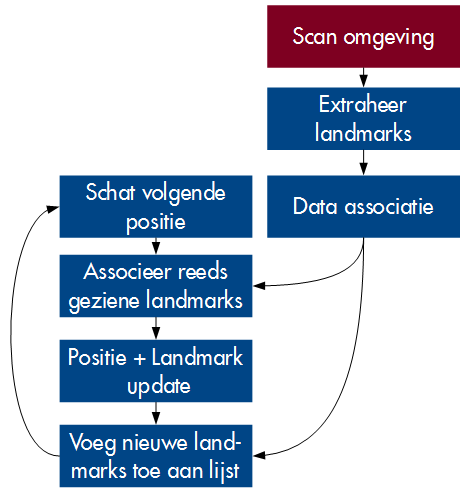
\includegraphics[width=0.5\linewidth]{SLAMprinciple}
	\caption{Grafische voorstelling van het basisalgoritme voor SLAM.} \label{fig:SLAMprin}
\end{figure}

\npar Bij iedere SLAM implementatie wordt een lijst aangelegd met zogenaamde \textit{landmarks}. Dit zijn referentiepunten, die in het geval van omgevingsmapping overeen stemmen met ofwel muurpunten ofwel obstakels in de ruimte die in kaart moet worden gebracht. Een quadcopter kan gebruik maken van de afstand tot de verschillende landmarks om zijn eigen positie te berekenen. Als nieuwe data beschikbaar is, worden hier eerst landmarks uit ge\"extraheerd. Op basis van de geschatte positie van het platform worden de ge\"extraheerde landmarks vergeleken met de reeds geziene landmarks. Deze vergelijking stelt het algoritme in staat de schatting te corrigeren door de positie van het platform en de landmarks te updaten. Eens de nieuwe positie gekend is, kan de locatie van de niet eerder geziene landmarks ook bepaald worden. Als het platform over odometrie beschikt, dan wordt dit vaak gebruikt om het schatten van de volgende positie nauwkeuriger te maken.

\npar De hierboven aangehaalde paradigma's verschillen in de manier waarop de nieuwe positie van de quadcopter en de positie van de landmarks wordt geschat.

\npar Voor de volledigheid wordt een derde paradigma vermeld. Graaf-gebaseerde optimalisatie technieken. Dit paradigma wordt in de praktijk zelden gebruikt voor online toepassingen en wordt daarom ook niet verder besproken \cite{book:SLAMHandbook}.

\subsection{Extended Kalman Filters}
De positie van de quadcopter en de positie van alle landmarks zijn allemaal stochastische variabelen. Er wordt verondersteld dat ze gemeenschappelijk gaussiaans verdeeld zijn. Een gaussiaanse verdeling met meerdere variabelen wordt getypeerd door een schatting van iedere variabele, de verwachtingswaarde en een schatting op de fout van die verwachtingswaarde, de covariantiematrix. Als een nieuwe scan beschikbaar is en er worden reeds geziene landmarks waargenomen, dan worden alle verwachtingswaarden en de volledige covariantiematrix ge\"updatet. Als er nieuwe landmarks worden gezien, dan worden die toegevoegd als extra variable aan de gaussiaanse verdeling. Het updaten van de verwachtingswaarden en de covariantiematrix, of anders verwoord het schatten van de nieuwe verwachtingswaarden en de covariantiematrix gebeurt aan de hand van Extended Kalman filters \cite{book:SLAMHandbook}.

\npar Het is zo dat EKF-SLAM na verloop van tijd altijd inconsistent wordt. Dit door het feit dat uitgegaan wordt van een gaussiaanse verdeling, terwijl de feitelijke verdeling voor de robotpositie en landmarks iets helemaal anders kan zijn \cite{paper:SLAMconsistency}.

\npar Om telkens opnieuw deze volledige covariantiematrix te updaten is veel rekenkracht nodig. Bovendien moeten ook voortdurend nieuwe landmarks worden toegevoegd wanneer nieuw terrein wordt verkend. Dit zorgt ervoor dat er nog meer berekeningen moeten gebeuren. Als antwoord op dit nadeel werd FastSLAM ontwikkeld \cite{paper:FastSLAM}. Dit is \'e\'en van de eerste SLAM algoritmes die gebruik maakt van particle filters \cite{paper:SLAMTutorial}.

\subsection{Particle Filters}
Het gebruik van particle filters voor het in kaart brengen van een onbekende omgeving werd ge\"introduceerd door K.P. Murphy \cite{paper:BayesianMap}. De eerste toepassing van zijn idee\"en volgde pas enkele jaren later met FastSLAM \cite{paper:FastSLAM}. De map en de positie van de quadcopter worden van elkaar losgekoppeld. Er worden meerdere partikels bijgehouden. Dit zijn als het ware mogelijke staten waarin het platform zich kan bevinden. Voor ieder partikel wordt een map bijgehouden. De punten worden opnieuw als guassiaans verdeeld ondersteld. Doordat de positie werd losgekoppeld van de map, zijn de landmarks niet langer afhankelijk van elkaar. Dit betekent dat ieder punt van een 2D map kan voorgesteld worden door een 2D verwachtingswaarde en een 2x2 covariantiematrix. Wanneer een nieuwe scan toekomt, wordt eerst de nieuwe positie geschat voor ieder partikel. Vervolgens wordt aan de hand van die schatting, voor ieder partikel de bijhorende verwachtingswaarde en covariantiematrix van alle landmarks ge\"updatet met een Kalman filter.

\npar Waar EKF-SLAM een gigantische matrix moest updaten, moet bij het gebruik van een particle filter, voor ieder partikel, voor iedere landmark de verwachtingswaarde en de covariantie matrix worden ge\"updatet. De complexiteit van de berekeningen bij een particle filter zullen dus lineair stijgen met het aantal landmarks. Bij EKF-SLAM stijgt de complexiteit kwadratisch. In FastSLAM worden landmarks dan nog eens georganiseerd in een boomstructuur. Dit zorgt ervoor dat complexiteit van de berekeningen logaritmisch schaalt met het aantal landmarks. Er kan besloten worden dat het gebruik van een particle filter een stuk minder zware berekeningen vergt \cite{paper:FastSLAM} \cite{book:SLAMHandbook}.

\subsection{Besluit}
Uit een korte literatuurstudie is gebleken dat er best geopteerd wordt voor een SLAM algoritme dat gebruik maakt van particle filters. Het is de bedoeling dat de map realtime gegenereerd wordt, dus de nodige rekenkracht moet beperkt blijven. Zeker omdat het uiteindelijk de bedoeling is het SLAM algoritme online op de quadcopter te laten draaien zodat het platform zelf kan beslissen naar waar gevlogen wordt om een volledige ruimte of misschien zelfs een volledig gebouw te verkennen. Hetzelfde besluit wordt gemaakt in werken gelijkaardig aan deze thesis \cite{paper:sameasme1} \cite{paper:sameasme2}.

\section{BreezySLAM}
Gezien de beperkte rekenkracht van het gebruikte platform is een algoritme dat gebruik maakt van particle filters aangewezen. Er zijn heel veel open source SLAM implementaties beschikbaar. Er wordt gezocht naar een implementatie die eenvoudig te verzoenen is met de architectuur van het platform in deze thesis. Bovendien wordt eerst gekeken naar SLAM implementaties die 2D mappen genereren. Pas wanneer het platform in staat is een goeie 2D map te maken, kan er gekeken worden of 3D mappen ook haalbaar zijn met de aanwezige hardware.

\npar \textit{HectorSLAM} wordt reeds gebruikt voor omgevingsmapping met een quadcopter in het werk van M. G\"abel et al. \cite{paper:sameasme1}\cite{paper:hectorSLAM}. Deze implementatie heeft als belangrijk voordeel dat er rekening wordt gehouden met de roll en pitch van het platform. Waarom dit belangrijk is wordt ge\"illustreerd in figuur \ref{fig:lasercomp}. Wanneer een quadcopter lichtjes kantelt, zijn de metingen van de laserscanner niet meer volledig correct. HectorSLAM is beschikbaar in het ROS raamwerk \cite{url:hectorROS}. Om HectorSLAM werkende te krijgen op de PC wordt op vrij veel problemen gestoten. Daarom wordt verder gezocht naar een andere implementatie.

\begin{figure}[h]
	\centering
	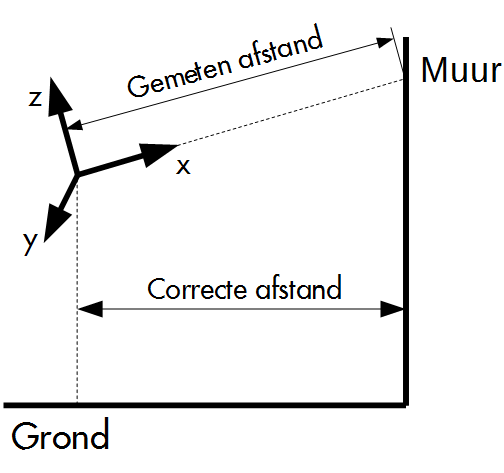
\includegraphics[width=0.40\linewidth]{lasercomp}
	\caption{Het assenstelsel op de figuur geeft de houding van een quadcopter weer. Er wordt ge\"illustreerd waarom de gemeten afstanden niet volledig kloppen wanneer het platform kantelt in een bepaalde richting.} \label{fig:lasercomp}
\end{figure}

\npar Wat wel makkelijk te integreren zou zijn is een implementatie die geschreven is in C of in Python, gezien deze twee talen reeds gebruikt werden voor het platform. Een zeer lichte C implementatie voor SLAM is \textit{TinySLAM} \cite{paper:tinySLAM} \cite{paper:tinySLAM2}. Zoals de naam al doet vermoeden, bestaat TinySLAM uit minder dan 200 lijnen code. Uit figuur \ref{fig:tinyslammap} blijkt het degelijk te presteren. Uiteindelijk wordt gekozen voor \textit{BreezySLAM} \cite{thesis:BreezySLAM} \cite{url:BreezySLAMlib}, een implementatie afgeleid van TinySLAM, omdat het een stuk gebruiksvriendelijker is. TinySLAM en BreezySLAM laten beide het gebruik van odometrie toe, maar roll en pitch horen daar niet bij. Er moeten dus maatregelen genomen worden om de roll en pitch te compenseren in de laserdata.

\begin{figure}[h]
	\centering
	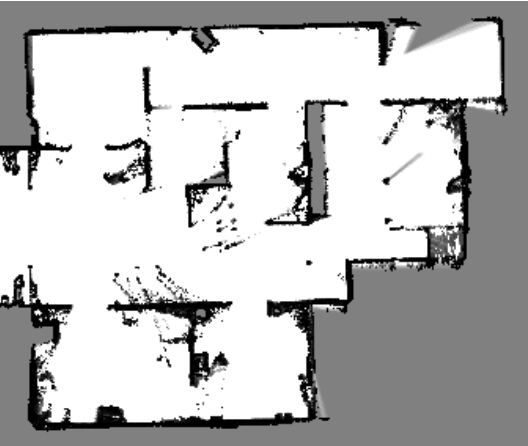
\includegraphics[width=0.31\linewidth]{tinySLAMmap}
	\caption{2D map gegenereerd met TinySLAM.} \label{fig:tinyslammap}
\end{figure}
